% !TeX program = xelatex
% !BIB program = biber

\documentclass[spanish]{textolivre}

% metadata
\journalname{Texto Livre}
\thevolume{18}
%\thenumber{1} % old template
\theyear{2025}
\receiveddate{\DTMdisplaydate{2024}{8}{1}{-1}}
\accepteddate{\DTMdisplaydate{2024}{10}{7}{-1}}
\publisheddate{\today}
\corrauthor{Javier Gil-Quintana}
\articledoi{10.1590/1983-3652.2024.53823}
%\articleid{NNNN} % if the article ID is not the last 5 numbers of its DOI, provide it using \articleid{} commmand 
% list of available sesscions in the journal: articles, dossier, reports, essays, reviews, interviews, editorial
\articlesessionname{articles}
\runningauthor{Gil-Quintana et al.}
%\editorname{Leonardo Araújo} % old template
\sectioneditorname{Daniervelin Pereira}
\layouteditorname{João Mesquita}

\title{Redes comunicativas universitarias sNOOC por la educación mediática de la tercera edad}
\othertitle{Redes de comunicação universitária sNOOC para educação midiática de idosos}
\othertitle{sNOOC communicative networks for media education of the elderly}

\author[1,2]{Javier Gil Quintana~\orcid{0000-0003-0326-2535}\thanks{Email: \href{mailto:jgilquintana@edu.uned.es}{jgilquintana@edu.uned.es}}}
\author[2]{Eduardo García Blázquez~\orcid{0000-0003-1229-3229}\thanks{Email: \href{mailto:ed.garcia@invi.uned.es}{ed.garcia@invi.uned.es}}}
\author[2]{José Javier Hueso Romero~\orcid{0000-0003-1375-2028}\thanks{Email: \href{mailto:jjavierhuesoromero@invi.uned.es}{jjavierhuesoromero@invi.uned.es}}}
\author[1]{Luis Miguel Romero Rodríguez~\orcid{0000-0003-3924-1517}\thanks{Email: \href{mailto:luis.romero@urjc.es}{luis.romero@urjc.es}}}
\affil[1]{Universidad Rey Juan Carlos, Facultad Ciencias de la Comunicación, Madrid, España.}
\affil[2]{Universidad Nacional de Educación a Distancia, Facultad de Educación, Madrid, España.}

\addbibresource{article.bib}

\begin{document}
\maketitle
\begin{polyabstract}
\begin{abstract}
Los Nano Open Online Massive (NOOC) representan una modalidad formativa de corta duración, análoga a los MOOC. Sin embargo, se caracterizan por una mayor especialización y brevedad, típicamente de 20 horas. El proyecto objeto de esta investigación aplicada, denominado socialNOOC (sNOOC), busca potenciar el empoderamiento del alumnado en su rol de e-teacher y evaluar el impacto de su labor en la educación mediática inclusiva de la población de la tercera edad en España. La iniciativa, coordinada por 79 estudiantes de posgrado de la UNED (España), se fundamenta en el proyecto formativo basado en pedagogías inclusivas en el que se integra recursos generados con Inteligencia Artificial y Metaverso. El análisis del proyecto ha incorporado enfoques cuantitativos, examinando las interacciones en la plataforma de educación a distancia (EAD) donde se desarrollaron los sNOOC, así como cualitativos, a través de la observación virtual de los 8 cursos masivos, las producciones de aprendizaje y la evaluación de un grupo interdisciplinario de 22 docentes en innovación educativa en España y Ecuador. Los resultados evidencian que la labor de los e-teacher e interacción de las redes comunicativas en los sNOOC han incrementado tanto el compromiso con el proyecto, como la satisfacción derivada de la experiencia colaborativa.

\keywords{Alfabetización informacional \sep Tercera edad \sep Educación a distancia. Metodología mixta}

\end{abstract}

\begin{portuguese}
\begin{abstract}
Nano Open Online Massive (NOOC) representa uma modalidade de treinamento de curta duração, análoga aos MOOCs. No entanto, caracterizam-se por maior especialização e brevidade, normalmente 20 horas. O projeto objeto desta investigação aplicada, denominado socialNOOC (sNOOC), procura potenciar a capacitação dos alunos no seu papel de e-professores e avaliar o impacto do seu trabalho na educação mediática inclusiva para a população idosa em Espanha. A iniciativa, coordenada por 79 alunos de pós-graduação da UNED (Espanha), baseia-se no projeto de formação baseado em pedagogias inclusivas em que se integram recursos gerados com Inteligência Artificial e Metaverso. A análise do projeto incorporou abordagens quantitativas, examinando as interações na plataforma de educação a distância (EAD) onde foram desenvolvidos os sNOOCs, e qualitativa, por meio da observação virtual dos 8 cursos massivos, das produções de aprendizagem e da avaliação de uma abordagem interdisciplinar. grupo de 22 professores em inovação educacional na Espanha e no Equador. Os resultados mostram que o trabalho dos e-professores e a interação das redes de comunicação no sNOOC aumentaram tanto o compromisso com o projeto como a satisfação derivada da experiência colaborativa.

\keywords{Alfabetização informacional\sep Terceira idade \sep Educação a Distância \sep Metodologia mista}

\end{abstract}
\end{portuguese}


\begin{english}
\begin{abstract}
Massive Nano Open Online Courses (MOOCs) are a short training modality similar to MOOCs, however they are characterized by greater specialization and brevity, usually lasting during the course of 20 hours. SocialNOOC (sNOOC) aims at empowering students to assume the role of e-teachers and assessing their contributions to the integrated media education of the elderly population in Spain through their work as e-teachers. This initiative is coordinated by 79 graduate students from the UNED (Spain) based on a training project integrating artificial intelligence and metaverse technology into pedagogical practices. Through the virtual observation of 8 massive courses, the learning productions, and the evaluation of an interdisciplinary group of 22 teaching experts in educational innovation in Spain and Ecuador, the project tters analyzed using quantitative approaches, examining interactions within the distance education platform (EAD), where the sNOOCs were developed, as well as qualitative approaches. The results show that the work of the e-teachers and the interaction of the communication networks in the sNOOCs have increased both the commitment to the project and the satisfaction derived from the collaborative experience.

\keywords{Information literacy \sep Third age \sep Distance education \sep Mixed methodology}
\end{abstract}
\end{english}
\end{polyabstract}

\section{Introducción}\label{sec-Introducción}

La evolución de la inteligencia artificial (IA) ha marcado un hito
significativo en la actualidad sofocada por infodemia e infoxicación.
Esta transformación tecnológica, inicialmente concebida por John
McCarthy en 1956, ha avanzado significativamente, incorporando
aplicaciones de aprendizaje automático y procesamiento del lenguaje
natural (NLP) en herramientas educativas \cite{Sadiku2021}. No obstante, el gran salto se dio con la presentación de
ChatGPT en 2020, y con mejor respuesta a principios del 2023, siendo la
IA Generativa (IAGen) otra forma de entender a la IA; la IAGen crea
contenido original a partir de datos existentes mediante algoritmos y
redes neuronales avanzadas \cite{Feuerriegel2024}.

En el campo de la educación, los modelos de lenguaje grandes (LLM,
\emph{Large Language Model}), como ChatGPT \cite{OpenAI2023}, ha generado
diversos debates públicos y digitales como el de la opinión emitida por
el lingüista {\textcite{Chomsky2023}}, donde califica a ChatGPT como una forma de plagio de alta
tecnología, pudiendo socavar la educación al motivar a los estudiantes
en la búsqueda de atajos para la entrega de trabajos, como los ya
clásicos ensayos o resolución a preguntas cerradas, como en un
cuestionario de reforzamiento, por ejemplo. Ante este tipo de
reflexiones, han surgido otras como la de \textcite{Yell2023}, un
profesor retirado de la Universidad de Wisconsin, argumentan sobre que,
si se utiliza de forma adecuada, ChatGPT puede ser un recurso valioso
para fomentar el aprendizaje basado en la búsqueda e investigación,
permitiendo promover el pensamiento crítico. Aunque es indiscutible que
este tipo de tecnología es capaz de crear contenido nuevo en formato de
texto, imágenes o audio, permitiendo hasta asistir en tareas de
conocimiento y necesidades cotidianas \cite{Feuerriegel2024}.

La aplicación de ChatGPT en la educación se ve reflejada en el análisis
de \textcite{Dimitriadou2023}, quienes abordan la integración de la
IA en las aulas inteligentes y los desafíos éticos asociados, así como
en el estudio de \textcite{Tlili2023} abordando el uso de
\emph{chatbots}, que examinan la aplicación de ChatGPT en la elaboración
de ejercicios en forma de cuestionarios. Estos enfoques resaltan el
equilibrio necesario entre las capacidades de la IA y la intervención
humana para garantizar la relevancia, la exactitud y la equidad en la
educación.

Recientes investigaciones, como las de \textcite{Nasution2023} y \textcite{Ruiz2023},
han explorado el uso de ChatGPT 4.0 en la generación de ítems de examen,
destacando no solo su capacidad para crear preguntas de elección
múltiple relevantes y coherentes, sino también abordando desafíos como
irregularidades y redundancias en interacciones más prolongadas. Estos
estudios subrayan la importancia de la especificidad y sistematización
en los prompts para generar exámenes eficientes y precisos,
capitalizando las fortalezas de la IA para la educación \cite{Nasution2023, Ruiz2023}.

La investigación de \textcite{Nasution2023} se enfocó en la validez y
confiabilidad de las preguntas generadas por IA, un tema que ha
suscitado tanto interés como preocupación en la comunidad educativa. Con
una muestra de 272 estudiantes, Nasution emprendió la tarea de evaluar
una serie de preguntas creadas por ChatGPT, obteniendo resultados que
son tanto prometedores como reveladores. De las 21 preguntas generadas
por la IA, 20 resultaron ser válidas, lo que indica una alta tasa de
éxito. Este hallazgo es significativo, ya que subraya la capacidad de la
IA para producir contenido educativo que no solo es relevante, sino
también de calidad.

No obstante, también hay investigaciones en torno al uso de Machine
Learning (ML) como el de \textcite{Rauber2024} quienes desarrollaron un
modelo automatizado para medir el aprendizaje de conceptos y prácticas
de clasificación de imágenes mediante redes neuronales. Se basó en datos
de 240 estudiantes de secundaria y bachillerato, concluyendo que la
evaluación es confiable y válida. Además, destacaron la efectividad del
modelo resaltando la importancia de incluir ML en la educación escolar y
la capacidad del modelo para asistir en el proceso de evaluación,
facilitando la carga de trabajo de los docentes.

A medida que la tecnología de IA continúa evolucionando, con avances
significativos en las versiones más recientes de ChatGPT, se presenta
una oportunidad única para mejorar y sistematizar el proceso de creación
de exámenes. Las investigaciones de \textcite{Nasution2023,Ruiz2023} se
alinean con esta visión, proponiendo un enfoque metodológico que combina
la exploración y descripción detallada de las capacidades de ChatGPT 4.0
en la generación de ítems de examen, proporcionando así una perspectiva
integral de su aplicabilidad y eficacia en el ámbito educativo. No
obstante, todavía hacen falta estudios que comparen el comportamiento de
la IAGen y si los seres humanos somos capaces de detectar esas
diferencias, o bien, podrían ayudar a reducir la carga de los docentes e
instituciones al momento de crear exámenes de alto impacto; como los del
ingreso a la universidad.

Ante todos estos acontecimientos, y retomando estos modelos de lenguaje
que podrían ayudarnos a evaluar nuestra propia forma de comunicar, el
objetivo principal de esta investigación fue explorar y comparar la
eficacia de la IAGen, representada por ChatGPT 4.0, y los diseñadores
humanos en el desarrollo de ítems para el Examen de Ingreso a la
Educación Superior (ExIES), en el área de Lengua Escrita, a través del
método de juicio de expertos. Lo anterior, con el fin determinar la
calidad, relevancia y alineación de los ítems generados por ambas
fuentes (IA y humanos) con los estándares establecidos para la
evaluación educativa, centrándose en aspectos como claridad,
neutralidad, concisión, alineación curricular y adecuación de formato y
contenido.
\section{Metodologia}\label{sec-metodologia}

Não foi necessária uma análise ética prévia por parte dos conselhos de
projetos adequados para a investigação, uma vez que os participantes não
foram identificados. Por não haver conflito de interesses, a Texto Livre
não terá quaisquer consequências, inclusive assistência integral e
eventual, ressarcimento de qualquer dano resultante a qualquer dos
participantes da pesquisa, conforme a Resolução nº 510, de 7 de abril de
2016, do Conselho Nacional de Saúde do Brasil.

A metodologia é a explicação minuciosa, detalhada, rigorosa e exata de
toda a ação desenvolvida no método de trabalho da pesquisa \cite{lakatos2003}. A pesquisa é um estudo de caso, que teve o aluno como
objeto de estudo. \textcite[p. 32]{yin2005} argumenta que o estudo de caso visa a \enquote{conhecer em profundidade o como e o porquê de uma determinada
	situação que se supõe ser única em muitos aspectos, procurando descobrir
	o que há nela de mais essencial e característico}. O estudo de caso é
caracterizado pelo estudo profundo e exaustivo de um ou poucos objetos,
de maneira a permitir o seu conhecimento amplo e detalhado. O caso
experimental caracteriza-se por determinar um objeto de estudo,
selecionar as variáveis que seriam capazes de influenciá-lo, definir as
formas de controle e de observação dos efeitos que a variável produz no
objeto \cite{gil2002}. A coleta dos dados foi realizada em uma escola
secundária do sul de Moçambique. Fizeram parte da amostra 50 alunos do
ensino secundário, selecionados de forma aleatória, dos quais 25
participaram do estudo das PO e aplicação do Q3DM. Os restantes 25
estiveram envolvidos no estudo das SCs e aplicação do GeoGebra. Em ambos
os estudos, todos os alunos experimentaram as aplicações (Q3DM ou
GeoGebra). A pesquisa apresenta um estudo de caso interpretativo, o qual
desenvolve categorias conceituais indutivamente para examinar os
pressupostos iniciais, as intenções e significados das ações e
expressões dos alunos \cite{amado2017}. A compreensão interpretativa é
sustentada a partir do relato pormenorizado da interação dos sujeitos em
seu meio natural \cite{coulon1995}. A visão interpretativa descreveu as
ações dos alunos em ambiente de sala de aula e os significados das ações
no processo de toda a pesquisa \cite{coutinho2011}.

Foi possível, pois, observar e interpretar tudo o que ocorreu, tornando
viável a análise das relações causa-efeito. Foi possível , também,
qualificar as ações dos alunos em todo o processo de aprendizagem, por
meio das interpretações dos significados de seus comportamentos durante
a mediação da aula e as respostas do questionário de satisfação. Além
disso, os dados foram coletados por meio das técnicas de observação do
participante, com tomada de notas e de registro fotográfico, assim como
dos instrumentos de coleta de dados aplicados, como os questionários de
satisfação.

\subsection{Realização das aulas}\label{sub-sec-Realização das aulas}

As aulas consistiram na apresentação de dois temas, PO e SCs, de forma
separada. Para os alunos da 9ª classe, o tema de pesquisa foi PO, e foi
utilizado o Q3DM. A professora primeiramente apresentou o tema,
explicando o que eram POs, dizendo que eram figuras geométricas sobre um
plano que poderiam ser comparadas à sombra do mesmo objeto no horário em
que o sol estaria no ponto mais alto no dia. Depois, demonstrou as
vistas ortogonais do sólido. (Ver \Cref{fig-03}).

\begin{figure}[htpb]
\centering
\begin{minipage}{.5\textwidth}
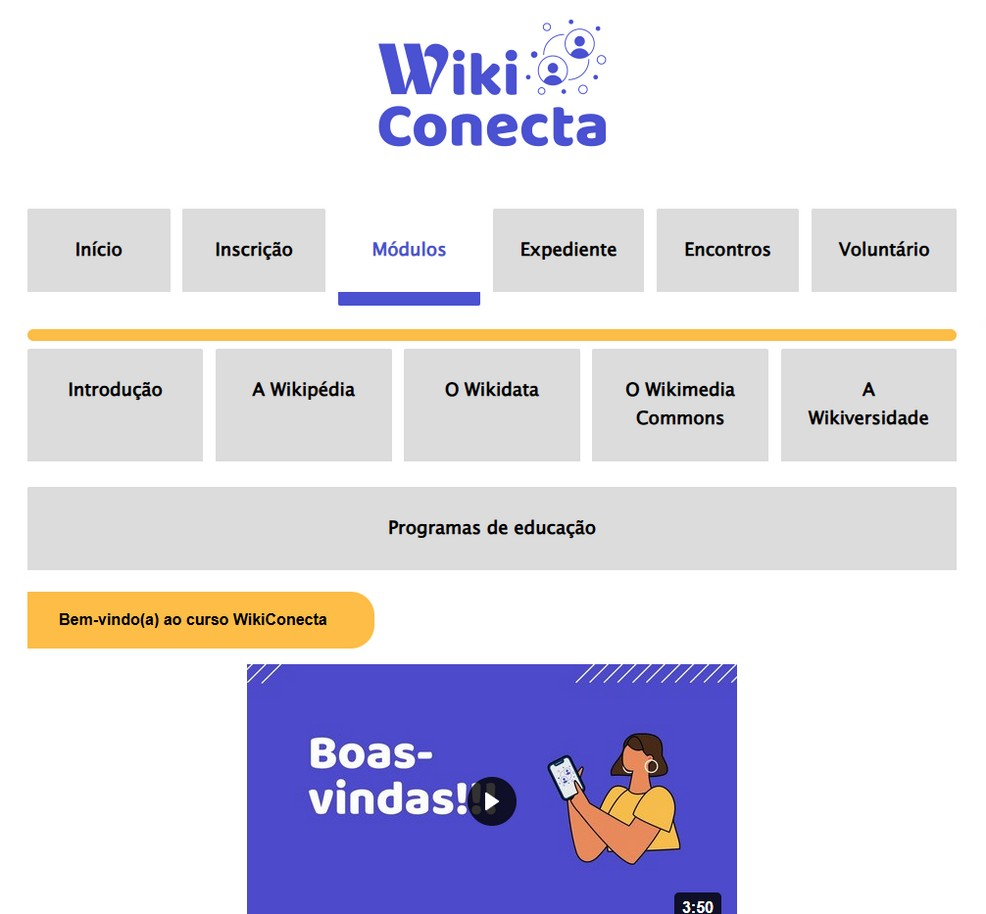
\includegraphics[width=\textwidth]{figures/figure03.jpg}
\caption{Vistas ortogonais e ortográficas: vista frontal; vista superior; e vista lateral esquerda.}
\label{fig-03}
\source{\url{http://turmag1215vialonga.blogspot.com/2014/10/projecoes-ortogonais.html}.}
\end{minipage}
\end{figure}

Posteriormente a professora apresentou a aplicabilidade das POs, dizendo
que eram destinadas à planificação de vários objetos. Com o auxílio das
simulações computacionais, construiu os sólidos geométricos e demonstrou
suas vistas ortogonais, apresentando os procedimentos para a manipulação
do Q3DM. (Ver \Cref{fig-04})

\begin{figure}[htpb]
\centering
\begin{minipage}{.5\textwidth}
\includegraphics[width=\textwidth]{figures/figure04.jpg}
\caption{Manipulação no Q3DM.}
\label{fig-04}
\source{Elaboração própria.}	
\end{minipage}
\end{figure}


A manipulação no Q3DM é feita por meio de cubos chamados Qubes, que
facilitam a criação e a montagem de objetos em três dimensões,
utilizando elementos digitais que podem ser inseridos, removidos,
deslocados, ampliados, inclinados, moldados geometricamente, girados e
coloridos.

Para os alunos da 12ª classe, o tema de pesquisa foi SCs e foi utilizado
o GeoGebra. A professora iniciou com a apresentação do tema SCs de
cilindro, explicando que a seção cilíndrica é uma figura resultante de
um plano secante no cilindro. A professora acrescentou que existem duas
situações distintas: quando o plano secante é paralelo ao eixo central
do cilindro; e quando o plano secante não é paralelo ao eixo central do
cilindro (ver as figuras \Cref{fig-05} e \Cref{fig-06}).

\begin{figure}[htpb]
\centering
\begin{minipage}{.25\textwidth}
\includegraphics[width=\textwidth]{figures/figure05.jpg}
\caption{Secção paralela ao eixo central do cilindro.}
\label{fig-05}
\source{Elaboração própria.}
\end{minipage}
\end{figure}

\begin{figure}[htpb]
\centering
\begin{minipage}{.5\textwidth}
\includegraphics[width=\textwidth]{figures/figure06.jpg}
\caption{Secção não paralela ao eixo central do cilindro.}
\label{fig-06}
\source{Elaboração própria.}
\end{minipage}
\end{figure}

A professora, primeiramente, apresentou os diferentes posicionamentos
dos planos em relação ao eixo central do cilindro. Em seguida, com o
auxílio da tecnologia, apresentou à turma o software de geometria
dinâmica GeoGebra, indicando as funcionalidades de suas ferramentas e
como construir do ponto até o plano secante, com a ajuda dos
procedimentos para a sua manipulação no GeoGebra. Os alunos simularam as
SCs com o plano de nível; eles apresentaram-se atentos e motivados em
aprender a resolver o exercício no GeoGebra, particularmente para os
rapazes, os quais procuravam descobrir como construir diferentes sólidos
geométricos e como simular as VOs (vistas ortogonais).

\subsection{Realização do questionário}\label{sub-sec-Realização do questionário}

O questionário de satisfação aplicado teve como objetivo compreender se
o Q3DM e o GeoGebra facilitaram a aprendizagem das POs e SCs, e se o
\textit{smartphone} foi fácil de manipular. Ambos os questionários foram
preenchidos em 10 minutos. As questões visavam a coletar, nos dois
estudos, várias opiniões, incluindo: (1) se os aplicativos tecnológicos
facilitaram as representações 3D; (2) qual é a opinião deles sobre os
benefícios de usar os aplicativos ou se seria melhor resolver de forma
tradicional; (3) se os aplicativos são fáceis e intuitivos de usar; (4)
quais foram os aspectos positivos e negativos da aula; e, (5) como eles
classificariam a aprendizagem com o auxílio dos aplicativos.

\section{Resultados e discussão}\label{sec-resultados}

Como dito anteriormente, foram feitos dois experimentos de classificação
de papéis semânticos. O primeiro envolve uma classificação binária (Arg0
e Arg1); já o segundo aborda uma classificação multiclasse com cinco
rótulos (Arg0, Arg1, Arg2, Arg3 e Arg4). Na \Cref{tab-03}, apresentamos os
resultados obtidos, considerando as medidas P, R, MF e A.

\begin{table}[htbp]
  \centering 
  \begin{threeparttable}
  \caption{Resultados para os dois experimentos de classificação.}
  \label{tab-03}
  \begin{tabular}{*{9}{l}}
  \toprule
  \multirow{2}{*}{CLASSES} & \multicolumn{8}{c}{EXPERIMENTOS} \\
    & \multicolumn{4}{c}{1º experimento (Arg0 e Arg1)} & \multicolumn{4}{c}{2º experimento (Arg0 a Arg4)} \\
    & P & R & MF & A & P & R & MF & A \\
  Arg0 & 0,83 & 0,82 & 0,82 & 0,85 & 0,82 & 0,79 & 0,81 & 0,76 \\
  Arg1 & 0,88 & 0,89 & 0,88 & 0,85 & 0,77 & 0,84 & 0,80 & 0,76 \\
  Arg2 &  -   &   -  &   -  &  -   & 0,40 & 0,32 & 0,36 & 0,76 \\
  Arg3 &  -   &   -  &   -  &  -   & 0,33 & 0,14 & 0,20 & 0,76 \\
  Arg4 &  -   &   -  &   -  &  -   & 1,00 & 0,20 & 0,33 & 0,76 \\
  \bottomrule
  \end{tabular}
  \source{Elaborado pelos autores.}
  \end{threeparttable}
\end{table}

Para o primeiro experimento, os resultados mostram um desempenho
equilibrado entre as duas classes. As métricas P, R e MF para Arg0 são,
respectivamente, 83\%, 82\% e 82\%, enquanto para Arg1 são 88\%, 89\% e
88\%. Esses resultados indicam um classificador bem balanceado,
sugerindo que o modelo consegue distinguir bem entre essas duas classes.

Por haver um aumento de classes, já era esperado um desbalanceamento na
performance do modelo entre as diferentes classes, no segundo
experimento. Para as classes Arg0 e Arg1, os resultados são semelhantes
aos do primeiro experimento, com MF de 81\% e 80\%, respectivamente. No
entanto, para as outras classes (Arg2, Arg3 e Arg4), as métricas são
significativamente mais baixas.

Para a classe Arg2, as medidas P, R e MF são 40\%, 32\% e 36\%,
respectivamente. A classe Arg4 apresenta uma precisão perfeita (100\%),
mas uma revocação extremamente baixa (20\%), resultando em uma MF de
apenas 33\%. A classe Arg3 também apresenta baixos valores em todas as
métricas, com precisão, revocação e medida F de 33\%, 14\% e 20\%,
respectivamente.

A acurácia de 76\% no segundo experimento sugere que o modelo tem uma
alta taxa de acertos nas classes majoritárias (Arg0 e Arg1), mas tem
dificuldade para classificar corretamente as classes minoritárias (Arg2,
Arg3 e Arg4), o que é evidenciado pelo baixo desempenho nestas classes.
Esse desbalanceamento indica que o modelo pode tender a classificar mais
exemplos nas classes majoritárias, possivelmente devido a um número
insuficiente de exemplos das classes minoritárias durante o treinamento.

Esse resultado pode ser justificado não apenas do ponto de vista
computacional, perpassado pelo desbalanceamento das classes, mas também
de uma perspectiva linguística. No primeiro experimento, consideraram-se
papéis de argumentos mais prototípicos e mais claramente associados a
posições sintáticas estabelecidas como sujeito e objeto, sendo mais
fáceis de se classificar. Já no segundo, observa-se uma diversidade
semântica e estrutural, sendo argumentos menos prototípicos, ocasionando
equívocos de classificação de predicados e adjuntos como argumentos.
Nesse caso, parece pertinente pontuar que é quase impossível desassociar
a estrutura argumental da sintaxe, cabendo mais discussões sobre essa
correlação em estudos posteriores.

Na língua geral, os papéis Arg0, Arg1 e Arg2 (como exemplificado em \ref{itm5a}, \ref{itm5b} e \ref{itm5c}, respectivamente) são mais profícuos, e os falantes constroem
rotineiramente sentenças que cumprem essas estruturas argumentais. Já as
construções que apresentam Arg3 e Arg4 (como exemplificado em \ref{itm5d} e \ref{itm5e},
respectivamente) seguem a proporção inversa. Destaca-se que os exemplos
demonstrados em \ref{itm5} foram extraídos do \emph{corpus little prince}, já
anotado com o modelo AMR, tendo a indicação do argumento correspondente
em foco.


\begin{enumerate}[start=5,label={(\arabic{enumi})}]
  \item\label{itm5}
    \begin{enumerate}[label=(\arabic{enumi}.\alph*)]
      \item\label{itm5a} {[}Ela{]}\textbf{\textsubscript{Arg0}} me perfumava.
      \item\label{itm5b} Perdoa-me {[}(eu){]}\textbf{\textsubscript{Arg1}}.
      \item\label{itm5c} Mas era tão {[}comovente!{ ]}\textbf{\textsubscript{Arg2}}
      \item\label{itm5d} {[}Perfura-o{]}\textbf{\textsubscript{Arg3}} com suas raízes.
      \item\label{itm5e} Vou passear até a {[}vinha.{]}\textbf{\textsubscript{Arg4}}
    \end{enumerate}
\end{enumerate}

É importante ressaltar que os predicados no modelo AMR equivalem à
descrição de uma ação, evento, estado ou relação e, por isso, são
frequentemente associados aos verbos, ainda que seja possível
associá-los a adjetivos e/ou substantivos. Além disso, frequentemente os
predicados correspondem a \emph{frames} semânticos, construindo cenas e
relações que exigem certos complementos. Já os argumentos são partícipes
ou entidades que se relacionam aos predicados, respondendo a perguntas
como ``quem'', ``o que?'' e ``para quem?'', por exemplo, sendo
enumerados em função da posição nos \emph{frames} em que são evocados.

Partindo desse princípio, os exemplos \ref{itm5a}, \ref{itm5b} e \ref{itm5e} cobrem essa
concepção; ainda que o quinto exemplo seja, na teoria linguística, um
argumento da preposição, na perspectiva da AMR ele é um argumento do
\emph{frame} ``passear''. Ao analisar os exemplos presentes em \ref{itm5c} e
\ref{itm5d}, evoca-se a necessidade de realizar revisões da anotação realizada.
Em \ref{itm5c}, ``comovente'' deveria ser considerado como predicado, mas
recebeu a anotação de argumento, pois completa o sentido de estado
(``ser comovente'', no caso). Já em \ref{itm5d}, o argumento deveria ser apenas
o objeto direto (no caso, ``o'') e não o verbo ``perfurar''. Esta última
colocação é justificada por uma questão de tokenização do \emph{corpus}
e do modelo de segmentação morfossintática utilizado, aglutinando o
``o'' a ``perfura''.

Ainda, em seus estudos, \textcite{cançado2009} encontrou predicados com no
máximo cinco lugares, como o verbo \emph{transportar} em ``João
transportou os livros no carro de São Paulo para a Bahia''. Nesse caso,
a autora admite que o complemento locativo ``no carro'' não é parte
obrigatória da estrutura argumental.

Nesse sentido, parece pertinente observar não apenas o quanto os
classificadores propostos acertam, mas também como se distribui o
equívoco de classificação no conjunto de dados. Por conta disso, foi
feita uma análise sobre a matriz de confusão dos modelos criados, em que
é possível avaliar a performance dos modelos em função de verdadeiros e
falsos positivos e negativos. Apresentamos as matrizes de confusão para
os dois experimentos nas \Cref{fig-04,fig-05}.


\begin{figure}[htpb]
\begin{minipage}{.45\textwidth}
  \centering
  \includegraphics[width=\textwidth]{figure04.jpg}
  \caption{Matriz de confusão do primeiro experimento}
  \label{fig-04}
  \source{Elaborado pelos autores.}
\end{minipage}%
\hfill
\begin{minipage}{.45\textwidth}
  \centering
  \includegraphics[width=\textwidth]{figure05.jpg}
  \caption{Matriz de confusão do segundo experimento}
  \label{fig-05}
  \source{Elaborado pelos autores.}
\end{minipage}
\end{figure}

As matrizes de confusão para os dois experimentos complementam as
métricas de avaliação apresentadas. No primeiro experimento, o modelo
mostra um bom equilíbrio entre P e R, com 179 (de 219) exemplos de Arg0
e 286 (de 323) exemplos de Arg1 corretamente classificados.

No segundo experimento, o modelo apresentou desequilíbrio em seu
desempenho. As classes Arg0 e Arg1 mantêm uma alta taxa de acerto, ao
passo que Arg2, Arg3 e Arg4 sofrem de baixa precisão e alta taxa de
erros. Essa confusão se deve ao fato de haver um desbalanceamento entre
os tipos de argumentos, conduzindo à classificação conforme a classe
majoritária, a saber, Arg1, conforme já discutido anteriormente.

Ainda, foi feita uma análise sobre o desempenho do modelo considerando
as classes e os \emph{corpora} utilizados nos dois experimentos.

\begin{table}[htpb]
  \centering
  \begin{threeparttable}
    \caption{Resultados do Experimento 1 em função dos \emph{corpora} utilizados.}
    \label{tab-04}
    \begin{tabular}{*{6}{l}}
      \toprule
      Corpora & Classe & P & R & MF & \multicolumn{1}{>{\raggedright\arraybackslash}p{2cm}}{Qnt. de instâncias} \\
      \midrule
      \arrayrulecolor[gray]{.7}
      \multirow{2}{*}{\emph{little prince}} 
        & Arg0 & 0,89 & 0,87 & 0,88 & 119 \\
        & Arg1 & 0,90 & 0,91 & \textbf{0,91} & 151 \\
      \midrule
      \multirow{2}{*}{\emph{news}} 
        & Arg0 & 0,74 & 0,75 & 0,74 & 60 \\
        & Arg1 & 0,87 & 0,86 & \textbf{0,87} & 116 \\
      \midrule
      \multirow{2}{*}{\emph{opisums}} 
        & Arg0 & 0,77 & 0,71 & 0,74 & 34 \\
        & Arg1 & 0,78 & 0,84 & \textbf{0,81} & 43 \\
      \midrule
      \multirow{2}{*}{\emph{sci}} 
        & Arg0 & 0,86 & 1,00 & 0,92 & 6 \\
        & Arg1 & 1,00 & 0,92 & \textbf{0,96} & 13 \\
      \arrayrulecolor{black}
      \bottomrule
    \end{tabular}
    \source{Elaborado pelos autores.}
  \end{threeparttable}
\end{table}

Na \Cref{tab-04}, relativa ao Experimento 1, observa-se que, considerando a
medida de avaliação MF, o modelo apresenta um melhor desempenho para
classificar Arg1 do que Arg0 para todos os \emph{corpora} utilizados.
Tal resultado pode ser explicado pela quantidade de instâncias
analisadas em Arg1 ser maior que Arg0. Ainda sobre a distribuição das
instâncias entre os \emph{corpora}, destaca-se que, apesar do
\emph{corpus sci} apresentar menos instâncias (no total, 19), o
\emph{corpus opisums} apresentou o menor desempenho com relação a MF, a
despeito da quantidade de instâncias (no total, 77). No entanto, é
possível notar que há um bom equilíbrio entre P e R para todos os
\emph{corpora}, indicando resultados consistentes para a classificação
do modelo.

\begin{table}[htpb]
  \centering
  \begin{threeparttable}
    \caption{Resultados do Experimento 2 em função dos \emph{corpora} utilizados.}
    \label{tab-05}
    \begin{tabular}{*{6}{l}}
      \toprule
      Corpora & Classe & P & R & MF & \multicolumn{1}{>{\raggedright\arraybackslash}p{2cm}}{Qnt. de instâncias} \\
      \midrule
      \arrayrulecolor[gray]{.7}
      \multirow{5}{*}{\emph{little prince}} 
        & Arg0 & 0,85 & 0,89 & \textbf{0,87} & 120 \\
        & Arg1 & 0,81 & 0,82 & 0,81 & 151 \\
        & Arg2 & 0,22 & 0,19 & 0,21 & 21 \\
        & Arg3 & 0,50 & 0,20 & 0,29 & 5 \\
        & Arg4 & 1,00 & 0,25 & 0,40 & 4 \\
      \midrule
      \multirow{5}{*}{\emph{news}} 
        & Arg0 & 0,77 & 0,68 & 0,73 & 60 \\
        & Arg1 & 0,74 & 0,86 & \textbf{0,80} & 115 \\
        & Arg2 & 0,57 & 0,39 & 0,46 & 31 \\
        & Arg3 & 0,00 & 0,00 & 0,00 & 1 \\
        & Arg4 & 0,00 & 0,00 & 0,00 & 1 \\
      \midrule
      \multirow{5}{*}{\emph{opisums}} 
        & Arg0 & 0,77 & 0,59 & 0,67 & 34 \\
        & Arg1 & 0,69 & 0,84 & \textbf{0,76} & 43 \\
        & Arg2 & 0,29 & 0,29 & 0,29 & 7 \\
        & Arg3 & 0,00 & 0,00 & 0,00 & 1 \\
        & Arg4 & 0,00 & 0,00 & 0,00 & 0 \\
      \midrule
      \multirow{5}{*}{\emph{sci}} 
        & Arg0 & 0,86 & 1,00 & \textbf{0,92} & 6 \\
        & Arg1 & 1,00 & 0,85 & \textbf{0,92} & 13 \\
        & Arg2 & 1,00 & 1,00 & \textbf{1,00} & 1 \\
        & Arg3 & 0,00 & 0,00 & 0,00 & 0 \\
        & Arg4 & 0,00 & 0,00 & 0,00 & 0 \\
      \arrayrulecolor{black}
      \bottomrule
    \end{tabular}
    \source{Elaborado pelos autores.}
  \end{threeparttable}
\end{table}


Na \cref{tab-05} relativa ao Experimento 2, observa-se que o Arg0 obteve um
melhor desempenho de classificação nos \emph{corpora} \emph{little
prince} e \emph{sci}, com MF de 0,87 e 0,92, respectivamente. Já Arg1
foi melhor classificado nos \emph{corpora news} e \emph{opisums}, com MF
de 0,88 e 0,76, respectivamente. Destaca-se também que no \emph{corpus
news}, Arg3 e Arg4 não foram classificados, apesar de ter um único
exemplo para cada uma dessas classes; o mesmo ocorre para Arg3 no
\emph{corpus opisums}. Em contrapartida,apenas uma única instância de
Arg2 no \emph{corpus sci} foi classificada corretamente pelo modelo.

Ainda com relação à \Cref{tab-05}, é possível inferir que as sentenças dos
\emph{corpora} podem apresentar estruturas argumentais distintas a
depender do domínio e/ou gênero textual a que se vinculam.

Além disso, foi feito um estudo sobre as \emph{features} mais relevantes
para a classificação dos papéis semânticos utilizando o método
\emph{feature importance}. Para tanto, somou-se a importância das
\emph{features} do Experimento 1 (\Cref{fig-06}) e do Experimento 2 (\Cref{fig-07}).

\begin{figure}[htpb]
  \centering
  \begin{minipage}{.75\textwidth}
  \includegraphics[width=\textwidth]{figure06.jpg}
  \caption{\emph{Features} mais relevantes para o Experimento 1.}
  \label{fig-06}
  \source{Elaborado pelos autores.}
  \end{minipage}
\end{figure}

\begin{figure}[htbp]
  \centering
  \begin{minipage}{.75\textwidth}
  
\includegraphics[width=\textwidth]{figure07.jpg}
  \caption{\emph{Features} mais relevantes para o Experimento 2.}
  \label{fig-07}
  \source{Elaborado pelos autores.}
  \end{minipage}
\end{figure}


Na \Cref{fig-06}, observa-se que os \emph{embeddings} dos lemas, tanto de
\emph{parent} quanto de \emph{child}, são particularmente significativos
para o modelo de classificação. No entanto, destaca-se que
\emph{embeddings} são as \emph{features} mais numerosas após a seleção.
Portanto, embora tenham uma grande soma de importância, individualmente,
sua relevância não é tão alta. Já na \Cref{fig-07}, além dos
\emph{embeddings} dos lemas, \emph{child\_tag}, \emph{child\_pos} e
\emph{dep} também se destacam. Nesse sentido, é possível inferir que, no
modelo criado, características de ordens morfossintáticas e sintáticas
são relevantes para a indicação dos papéis semânticos. Ressalta-se que
este tipo de observação é relevante em análises futuras, indicando quais
\emph{features} são mais relevantes em tarefas como a que foi
desenvolvida neste trabalho, além de contrapor o modelo teórico AMR que,
em tese, exclui esses níveis de conhecimento linguístico na
representação do significado e de sua estrutura argumental.

Por fim, foi empregado o método de \emph{shap values} para uma análise
mais profunda. Nesse método, conseguimos analisar como cada
\emph{feature} performa em função dos papéis semânticos observados. É
importante destacar que tal método se difere do
\emph{feature\_importance} por considerar a interação entre as
\emph{features} e a sua influência nas predições específicas. Vale
ressaltar que utilizamos apenas os \emph{shap values} para o conjunto de
treino, tendo em vista que o objetivo da análise é entender quais
padrões o modelo entendeu no seu treinamento como sendo mais
importantes. Para tanto, somaram-se os \emph{shap values} absolutos para
cada uma das \emph{features} originais e tirou-se a média de todas as
instâncias agrupadas pelo argumento para o Experimento 1 (\Cref{fig-08}) e o Experimento 2 (\Cref{fig-09}).

\begin{figure}[htpb]
  \centering
  \begin{minipage}{.75\textwidth}
  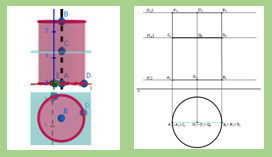
\includegraphics[width=\textwidth]{figure08.jpg}
  \caption{\emph{Features} mais relevantes para o Experimento 1 em função dos argumentos utilizando \emph{shap values}.}
  \label{fig-08}
  \source{Elaborado pelos autores.}
  \end{minipage}
\end{figure}

\begin{figure}[htbp]
  \centering
  \begin{minipage}{.75\textwidth}
  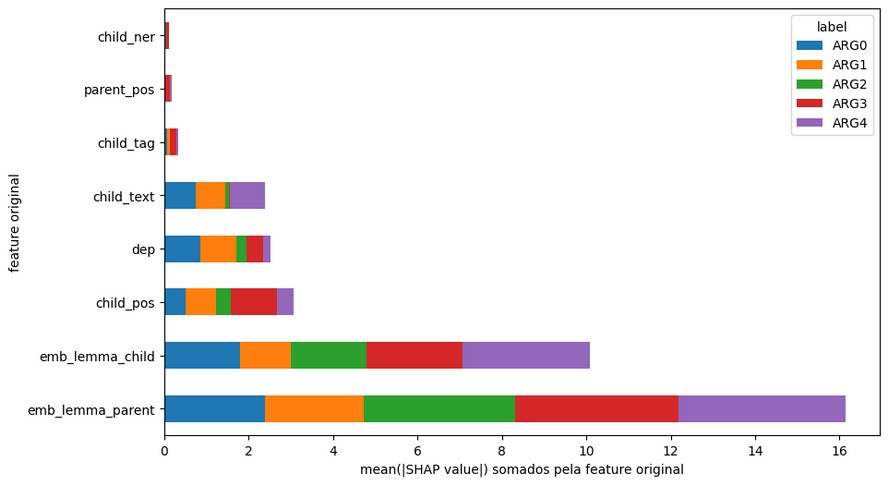
\includegraphics[width=\textwidth]{figure09.jpg}
  \caption{\emph{Features} mais relevantes para o Experimento 2 em função dos argumentos utilizando \emph{shap values}.}
  \label{fig-09}
  \source{Elaborado pelos autores.}
  \end{minipage}
\end{figure}


Na \Cref{fig-08}, evidencia-se que \emph{emb\_lemma\_parent} tem
discretamente maior relevância na classificação automática para Arg1 do
que Arg2, o que é inversamente proporcional para \emph{dep} e
\emph{emb\_lemma\_child}. Quanto a \emph{child\_tag}, \emph{child\_ner}
e \emph{child\_pos}, a relevância é bem baixa nesse cenário para as duas
classes analisadas; ao passo que \emph{parent\_pos} e \emph{parent\_tag}
não apresentaram qualquer relevância para nenhum dos dois papéis
semânticos. Quando o cenário de classificação é ampliado para os Args 0
a 4, o classificador recorre a algumas \emph{features} diferentes
daquelas utilizadas no primeiro experimento. Na \Cref{fig-09}, em especial,
tem-se que \emph{emb\_lemma\_parent} e \emph{emb\_lemma\_child} foram as
\emph{features} com maior relevância na classificação dos papéis
semânticos, sobretudo entre as classes Arg2, Arg3 e Arg4; ao passo que
\emph{child\_text}, que no experimento anterior não havia sido
utilizada, apresenta maior impacto para Arg0, Arg1 e Arg4.
\section{Discusión y Conclusiones}\label{sec-DiscusiónyConclusiones}

El uso e investigación del uso de la IAGen se encuentra en un momento
crucial de la historia educativa. Este estudio no solo se alinea con la
evolución tecnológica en la educación, sino que también aborda la
intersección de la IA y las metodologías de evaluación, un tema que ya
ha capturado la atención de académicos y educadores por igual \cite{Sadiku2021,Hosseini2023}. Esto a pesar de la discusión pública
sobre el papel de ChatGPT en la educación, marcada por voces críticas
como \textcite{Chomsky2023}, que contrasta con perspectivas
más optimistas como la de\textcite{Yell2023}, quien subraya el potencial de la
IAGen para enriquecer el aprendizaje.

Uno de estos ejemplos es la capacidad de ChatGPT para generar ítems de
examen válidos y relevantes, como se demostró en la investigación de
\textcite{Nasution2023}, refleja un avance hacia la automatización en la
creación de contenido educativo, respaldando los argumentos de eficacia
y eficiencia en la utilización de tecnologías avanzadas en la educación
\cite{Feuerriegel2024,Dimitriadou2023,Tlili2023}. Este estudio trata de abonar a esta visión optimista de \textcite{Yell2023} y \textcite{Nasution2023} sobre el uso e inclusión de la IAGen en procesos educativos.

Los resultados obtenidos sugieren que, bajo un juicio de expertos
cuidadosamente diseñado, los ítems generados por ChatGPT alcanzan un
nivel de aceptación comparable a los creados por humanos. Este hallazgo
es consistente con las observaciones de \textcite{Rauber2024}, quienes
también destacaron la utilidad de la tecnología de aprendizaje
automático en la evaluación educativa. Sin embargo, la variabilidad en
la aceptación de ítems entre los diseñadores humanos y ChatGPT resalta
la importancia de la supervisión humana y la necesidad de ajustes
específicos para alinear los ítems generados por IA con los estándares
educativos \cite{Nasution2023, Ruiz2023}.

Las contribuciones de este estudio se centran en demostrar el potencial
de la IAGen para asistir en la creación de contenido educativo validado,
al tiempo que se subraya la necesidad de un marco de juicio de expertos
robusto para evaluar la calidad de este contenido. A pesar de los
resultados prometedores sobre la no diferencia de comportamiento entre
jueces humanos y ChatGPT, existen limitaciones inherentes al estudio,
como la dependencia de la especificidad de los \emph{prompts} y la
variabilidad en la capacidad de juicio de los expertos, lo que sugiere
la necesidad de una investigación futura para optimizar los procesos de
generación y evaluación de ítems con IAGen, sobre todo debido a los
resultados de la confiabilidad inter-jueces, que a pesar de ser
positivos para el ChatGPT, hubo discordancia entre los jueces humanos
\cite{Galicia2017}.

Finalmente, este estudio no solo refuerza la viabilidad de utilizar
ChatGPT y otras tecnologías de IAGen en la educación, sino que también
destaca la importancia crítica del juicio humano experto en la
validación de contenido generado por IA. Al vincular estrechamente los
hallazgos con los objetivos planteados, este trabajo contribuye
significativamente a la discusión sobre el equilibrio entre la
innovación tecnológica y la necesidad de mantener altos estándares de
calidad y relevancia en la educación. La investigación futura debería
centrarse en perfeccionar la sinergia entre la inteligencia artificial y
el juicio humano para maximizar los beneficios de ambas en el desarrollo
educativo.

Algunos estudios posteriores:

\begin{itemize}
\item Se dará seguimiento a la evaluación de los ítems, comparando los desarrollados por humanos y por ChatGPT; se puede adelantar que los ítems se muestran consistentes, pero será publicado posteriormente (\Cref{appdx1}).
\item Se dará seguimiento y se seguirán desarrollando este tipo de ítems con IAGen para observar sus limitaciones y posibles aportes importantes; recordando que hay constantes actualizaciones de ChatGPT y similares.
\end{itemize}
\section{Conclusión}\label{sec-conclusión}

Las redes comunicativas sNOOC constituidas desde la formación de
posgrado y formadas por estudiantes que pasan a ser \emph{e-teacher} son
un ejemplo más de esfuerzo por la educación mediática inclusiva, en este
caso concreto, de la tercera edad. Gracias a plataformas como la de la
UNED, tmooc.es y el modelo sNOOC, se ha conseguido incentivar un modelo
formativo que pone de manifiesto un acceso equitativo y una
participación en la construcción colectiva del conocimiento. Esta
propuesta innovadora ha ayudado a consolidar un enfoque educativo y
comunicativo inclusivo adaptado a sectores vulnerables, a pesar de las
limitaciones del estudio como el tamaño de la muestra y la concreción de
los resultados en un contexto universitario determinado. La valoración
positiva de la experiencia formativa que hemos prestado en este artículo
no sólo destaca por su planteamiento didáctico o por la interacción de
las redes comunicativas creadas, sino que subraya el papel central de la
alfabetización mediática en la inclusión social de personas de la
tercera edad.

Es clave, como perspectiva futura, seguir fomentando la creación y
posterior investigación de redes comunicativas sNOOC, que asienten sus
proyectos formativos en acciones colaborativas y solidarias, potenciando
el uso de la inteligencia artificial, la gamificación y los entornos
inmersivos integrados en una pedagogía inclusiva. En un momento clave
para la formación a distancia, el reto de los agentes educativos y
sociales que se unen en red será mantener y mejorar la calidad del
modelo comunicativo y pedagógico, asegurando unas plataformas de
calidad, accesibles, adaptables y centradas en una comunicación
horizontal y bidireccional.

\printbibliography\label{sec-bib}
%conceptualization,datacuration,formalanalysis,funding,investigation,methodology,projadm,resources,software,supervision,validation,visualization,writing,review
\begin{contributors}[sec-contributors]
\authorcontribution{Javier Gil Quintana}[conceptualization,investigation,methodology,formalanalysis,writing,review] 
\authorcontribution{Eduardo García Blázquez}[datacuration,formalanalysis]
\authorcontribution{José Javier Hueso Romero}[conceptualization,supervision,review]
\authorcontribution{Luis Miguel Romero Rodríguez}[supervision,review]
\end{contributors}
\end{document}
